\documentclass[1p]{elsarticle_modified}
%\bibliographystyle{elsarticle-num}

%\usepackage[colorlinks]{hyperref}
%\usepackage{abbrmath_seonhwa} %\Abb, \Ascr, \Acal ,\Abf, \Afrak
\usepackage{amsfonts}
\usepackage{amssymb}
\usepackage{amsmath}
\usepackage{amsthm}
\usepackage{scalefnt}
\usepackage{amsbsy}
\usepackage{kotex}
\usepackage{caption}
\usepackage{subfig}
\usepackage{color}
\usepackage{graphicx}
\usepackage{xcolor} %% white, black, red, green, blue, cyan, magenta, yellow
\usepackage{float}
\usepackage{setspace}
\usepackage{hyperref}

\usepackage{tikz}
\usetikzlibrary{arrows}

\usepackage{multirow}
\usepackage{array} % fixed length table
\usepackage{hhline}

%%%%%%%%%%%%%%%%%%%%%
\makeatletter
\renewcommand*\env@matrix[1][\arraystretch]{%
	\edef\arraystretch{#1}%
	\hskip -\arraycolsep
	\let\@ifnextchar\new@ifnextchar
	\array{*\c@MaxMatrixCols c}}
\makeatother %https://tex.stackexchange.com/questions/14071/how-can-i-increase-the-line-spacing-in-a-matrix
%%%%%%%%%%%%%%%

\usepackage[normalem]{ulem}

\newcommand{\msout}[1]{\ifmmode\text{\sout{\ensuremath{#1}}}\else\sout{#1}\fi}
%SOURCE: \msout is \stkout macro in https://tex.stackexchange.com/questions/20609/strikeout-in-math-mode

\newcommand{\cancel}[1]{
	\ifmmode
	{\color{red}\msout{#1}}
	\else
	{\color{red}\sout{#1}}
	\fi
}

\newcommand{\add}[1]{
	{\color{blue}\uwave{#1}}
}

\newcommand{\replace}[2]{
	\ifmmode
	{\color{red}\msout{#1}}{\color{blue}\uwave{#2}}
	\else
	{\color{red}\sout{#1}}{\color{blue}\uwave{#2}}
	\fi
}

\newcommand{\Sol}{\mathcal{S}} %segment
\newcommand{\D}{D} %diagram
\newcommand{\A}{\mathcal{A}} %arc


%%%%%%%%%%%%%%%%%%%%%%%%%%%%%5 test

\def\sl{\operatorname{\textup{SL}}(2,\Cbb)}
\def\psl{\operatorname{\textup{PSL}}(2,\Cbb)}
\def\quan{\mkern 1mu \triangleright \mkern 1mu}

\theoremstyle{definition}
\newtheorem{thm}{Theorem}[section]
\newtheorem{prop}[thm]{Proposition}
\newtheorem{lem}[thm]{Lemma}
\newtheorem{ques}[thm]{Question}
\newtheorem{cor}[thm]{Corollary}
\newtheorem{defn}[thm]{Definition}
\newtheorem{exam}[thm]{Example}
\newtheorem{rmk}[thm]{Remark}
\newtheorem{alg}[thm]{Algorithm}

\newcommand{\I}{\sqrt{-1}}
\begin{document}

%\begin{frontmatter}
%
%\title{Boundary parabolic representations of knots up to 8 crossings}
%
%%% Group authors per affiliation:
%\author{Yunhi Cho} 
%\address{Department of Mathematics, University of Seoul, Seoul, Korea}
%\ead{yhcho@uos.ac.kr}
%
%
%\author{Seonhwa Kim} %\fnref{s_kim}}
%\address{Center for Geometry and Physics, Institute for Basic Science, Pohang, 37673, Korea}
%\ead{ryeona17@ibs.re.kr}
%
%\author{Hyuk Kim}
%\address{Department of Mathematical Sciences, Seoul National University, Seoul 08826, Korea}
%\ead{hyukkim@snu.ac.kr}
%
%\author{Seokbeom Yoon}
%\address{Department of Mathematical Sciences, Seoul National University, Seoul, 08826,  Korea}
%\ead{sbyoon15@snu.ac.kr}
%
%\begin{abstract}
%We find all boundary parabolic representation of knots up to 8 crossings.
%
%\end{abstract}
%\begin{keyword}
%    \MSC[2010] 57M25 
%\end{keyword}
%
%\end{frontmatter}

%\linenumbers
%\tableofcontents
%
\newcommand\colored[1]{\textcolor{white}{\rule[-0.35ex]{0.8em}{1.4ex}}\kern-0.8em\color{red} #1}%
%\newcommand\colored[1]{\textcolor{white}{ #1}\kern-2.17ex	\textcolor{white}{ #1}\kern-1.81ex	\textcolor{white}{ #1}\kern-2.15ex\color{red}#1	}

{\Large $\underline{12n_{0528}~(K12n_{0528})}$}

\setlength{\tabcolsep}{10pt}
\renewcommand{\arraystretch}{1.6}
\vspace{1cm}\begin{tabular}{m{100pt}>{\centering\arraybackslash}m{274pt}}
\multirow{5}{120pt}{
	\centering
	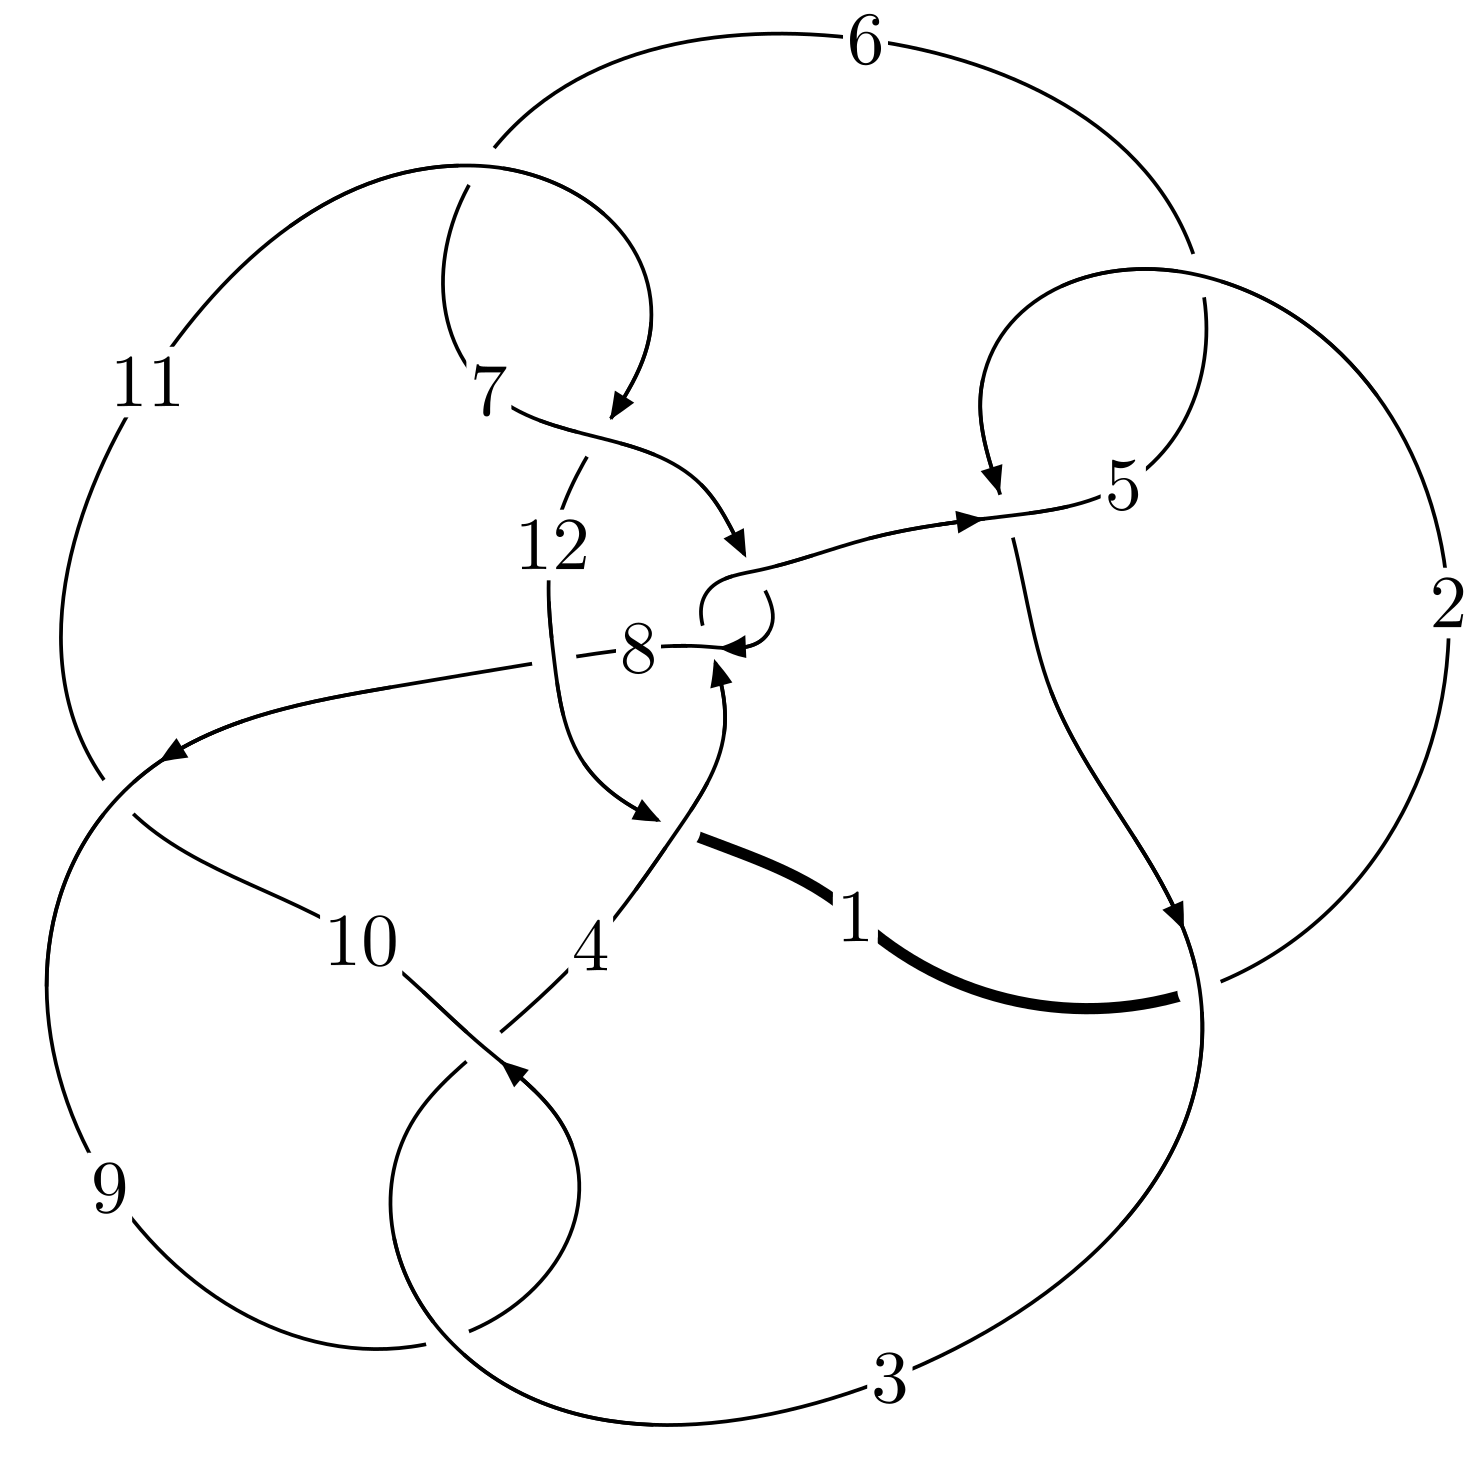
\includegraphics[width=112pt]{../../../GIT/diagram.site/Diagrams/png/2617_12n_0528.png}\\
\ \ \ A knot diagram\footnotemark}&
\allowdisplaybreaks
\textbf{Linearized knot diagam} \\
\cline{2-2}
 &
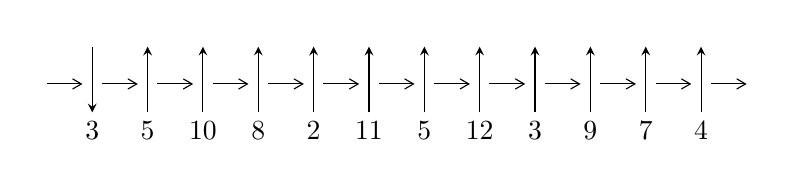
\begin{tikzpicture}[x=20pt, y=17pt]
	% nodes
	\node (C0) at (0, 0) {};
	\node (C1) at (1, 0) {};
	\node (C1U) at (1, +1) {};
	\node (C1D) at (1, -1) {3};

	\node (C2) at (2, 0) {};
	\node (C2U) at (2, +1) {};
	\node (C2D) at (2, -1) {5};

	\node (C3) at (3, 0) {};
	\node (C3U) at (3, +1) {};
	\node (C3D) at (3, -1) {10};

	\node (C4) at (4, 0) {};
	\node (C4U) at (4, +1) {};
	\node (C4D) at (4, -1) {8};

	\node (C5) at (5, 0) {};
	\node (C5U) at (5, +1) {};
	\node (C5D) at (5, -1) {2};

	\node (C6) at (6, 0) {};
	\node (C6U) at (6, +1) {};
	\node (C6D) at (6, -1) {11};

	\node (C7) at (7, 0) {};
	\node (C7U) at (7, +1) {};
	\node (C7D) at (7, -1) {5};

	\node (C8) at (8, 0) {};
	\node (C8U) at (8, +1) {};
	\node (C8D) at (8, -1) {12};

	\node (C9) at (9, 0) {};
	\node (C9U) at (9, +1) {};
	\node (C9D) at (9, -1) {3};

	\node (C10) at (10, 0) {};
	\node (C10U) at (10, +1) {};
	\node (C10D) at (10, -1) {9};

	\node (C11) at (11, 0) {};
	\node (C11U) at (11, +1) {};
	\node (C11D) at (11, -1) {7};

	\node (C12) at (12, 0) {};
	\node (C12U) at (12, +1) {};
	\node (C12D) at (12, -1) {4};
	\node (C13) at (13, 0) {};

	% arrows
	\draw[->,>={angle 60}]
	(C0) edge (C1) (C1) edge (C2) (C2) edge (C3) (C3) edge (C4) (C4) edge (C5) (C5) edge (C6) (C6) edge (C7) (C7) edge (C8) (C8) edge (C9) (C9) edge (C10) (C10) edge (C11) (C11) edge (C12) (C12) edge (C13) ;	\draw[->,>=stealth]
	(C1U) edge (C1D) (C2D) edge (C2U) (C3D) edge (C3U) (C4D) edge (C4U) (C5D) edge (C5U) (C6D) edge (C6U) (C7D) edge (C7U) (C8D) edge (C8U) (C9D) edge (C9U) (C10D) edge (C10U) (C11D) edge (C11U) (C12D) edge (C12U) ;
	\end{tikzpicture} \\
\hhline{~~} \\& 
\textbf{Solving Sequence} \\ \cline{2-2} 
 &
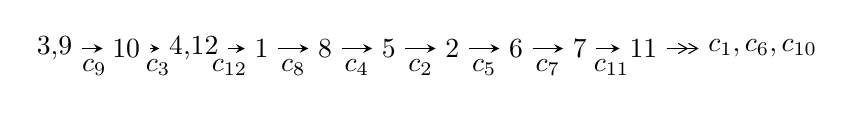
\begin{tikzpicture}[x=23pt, y=7pt]
	% node
	\node (A0) at (-1/8, 0) {3,9};
	\node (A1) at (1, 0) {10};
	\node (A2) at (33/16, 0) {4,12};
	\node (A3) at (25/8, 0) {1};
	\node (A4) at (33/8, 0) {8};
	\node (A5) at (41/8, 0) {5};
	\node (A6) at (49/8, 0) {2};
	\node (A7) at (57/8, 0) {6};
	\node (A8) at (65/8, 0) {7};
	\node (A9) at (73/8, 0) {11};
	\node (C1) at (1/2, -1) {$c_{9}$};
	\node (C2) at (3/2, -1) {$c_{3}$};
	\node (C3) at (21/8, -1) {$c_{12}$};
	\node (C4) at (29/8, -1) {$c_{8}$};
	\node (C5) at (37/8, -1) {$c_{4}$};
	\node (C6) at (45/8, -1) {$c_{2}$};
	\node (C7) at (53/8, -1) {$c_{5}$};
	\node (C8) at (61/8, -1) {$c_{7}$};
	\node (C9) at (69/8, -1) {$c_{11}$};
	\node (A10) at (11, 0) {$c_{1},c_{6},c_{10}$};

	% edge
	\draw[->,>=stealth]	
	(A0) edge (A1) (A1) edge (A2) (A2) edge (A3) (A3) edge (A4) (A4) edge (A5) (A5) edge (A6) (A6) edge (A7) (A7) edge (A8) (A8) edge (A9) ;
	\draw[->>,>={angle 60}]	
	(A9) edge (A10);
\end{tikzpicture} \\ 

\end{tabular} \\

\footnotetext{
The image of knot diagram is generated by the software ``\textbf{Draw programme}" developed by Andrew Bartholomew(\url{http://www.layer8.co.uk/maths/draw/index.htm\#Running-draw}), where we modified some parts for our purpose(\url{https://github.com/CATsTAILs/LinksPainter}).
}\phantom \\ \newline 
\centering \textbf{Ideals for irreducible components\footnotemark of $X_{\text{par}}$} 
 
\begin{align*}
I^u_{1}&=\langle 
-4.69351\times10^{67} u^{41}+3.55947\times10^{66} u^{40}+\cdots+1.96775\times10^{68} b-6.12388\times10^{68},\\
\phantom{I^u_{1}}&\phantom{= \langle  }8.52173\times10^{68} u^{41}+2.62218\times10^{67} u^{40}+\cdots+2.16453\times10^{69} a-5.80462\times10^{68},\;u^{42}- u^{41}+\cdots+7 u-11\rangle \\
I^u_{2}&=\langle 
- u^{23}+6 u^{21}+\cdots+b+1,\;2 u^{23}-13 u^{21}+\cdots+a-8,\;u^{24}-7 u^{22}+\cdots+2 u+1\rangle \\
\\
\end{align*}
\raggedright * 2 irreducible components of $\dim_{\mathbb{C}}=0$, with total 66 representations.\\
\footnotetext{All coefficients of polynomials are rational numbers. But the coefficients are sometimes approximated in decimal forms when there is not enough margin.}
\newpage
\renewcommand{\arraystretch}{1}
\centering \section*{I. $I^u_{1}= \langle -4.69\times10^{67} u^{41}+3.56\times10^{66} u^{40}+\cdots+1.97\times10^{68} b-6.12\times10^{68},\;8.52\times10^{68} u^{41}+2.62\times10^{67} u^{40}+\cdots+2.16\times10^{69} a-5.80\times10^{68},\;u^{42}- u^{41}+\cdots+7 u-11 \rangle$}
\flushleft \textbf{(i) Arc colorings}\\
\begin{tabular}{m{7pt} m{180pt} m{7pt} m{180pt} }
\flushright $a_{3}=$&$\begin{pmatrix}0\\u\end{pmatrix}$ \\
\flushright $a_{9}=$&$\begin{pmatrix}1\\0\end{pmatrix}$ \\
\flushright $a_{10}=$&$\begin{pmatrix}1\\- u^2\end{pmatrix}$ \\
\flushright $a_{4}=$&$\begin{pmatrix}u\\- u^3+u\end{pmatrix}$ \\
\flushright $a_{12}=$&$\begin{pmatrix}-0.393699 u^{41}-0.0121143 u^{40}+\cdots+3.32268 u+0.268170\\0.238522 u^{41}-0.0180890 u^{40}+\cdots-1.02660 u+3.11212\end{pmatrix}$ \\
\flushright $a_{1}=$&$\begin{pmatrix}0.0278896 u^{41}-0.0937965 u^{40}+\cdots+3.36008 u+4.84817\\0.449875 u^{41}+0.0226937 u^{40}+\cdots-3.24732 u+3.95315\end{pmatrix}$ \\
\flushright $a_{8}=$&$\begin{pmatrix}-0.270147 u^{41}-0.104563 u^{40}+\cdots+1.82540 u-2.97138\\-0.123129 u^{41}+0.000949344 u^{40}+\cdots-2.15974 u-3.88780\end{pmatrix}$ \\
\flushright $a_{5}=$&$\begin{pmatrix}-0.173180 u^{41}-0.00979843 u^{40}+\cdots+0.668036 u-2.62647\\0.153388 u^{41}-0.142217 u^{40}+\cdots+7.32309 u+5.63335\end{pmatrix}$ \\
\flushright $a_{2}=$&$\begin{pmatrix}0.0278896 u^{41}-0.0937965 u^{40}+\cdots+3.36008 u+4.84817\\0.296249 u^{41}+0.0542077 u^{40}+\cdots-2.47919 u+3.22817\end{pmatrix}$ \\
\flushright $a_{6}=$&$\begin{pmatrix}-0.413508 u^{41}+0.339840 u^{40}+\cdots-8.97780 u-9.77944\\-0.0992743 u^{41}-0.0250768 u^{40}+\cdots+3.47552 u+1.40486\end{pmatrix}$ \\
\flushright $a_{7}=$&$\begin{pmatrix}0.363292 u^{41}-0.398230 u^{40}+\cdots+9.99588 u+9.98935\\0.236749 u^{41}-0.0235247 u^{40}+\cdots-2.79328 u+0.767418\end{pmatrix}$ \\
\flushright $a_{11}=$&$\begin{pmatrix}- u^2+1\\- u^2\end{pmatrix}$\\&\end{tabular}
\flushleft \textbf{(ii) Obstruction class $= -1$}\\~\\
\flushleft \textbf{(iii) Cusp Shapes $= 3.35147 u^{41}-0.742817 u^{40}+\cdots+14.9249 u+57.1841$}\\~\\
\newpage\renewcommand{\arraystretch}{1}
\flushleft \textbf{(iv) u-Polynomials at the component}\newline \\
\begin{tabular}{m{50pt}|m{274pt}}
Crossings & \hspace{64pt}u-Polynomials at each crossing \\
\hline $$\begin{aligned}c_{1}\end{aligned}$$&$\begin{aligned}
&u^{42}+64 u^{41}+\cdots-29237998 u+1857769
\end{aligned}$\\
\hline $$\begin{aligned}c_{2},c_{5}\end{aligned}$$&$\begin{aligned}
&u^{42}+2 u^{41}+\cdots-2362 u-1363
\end{aligned}$\\
\hline $$\begin{aligned}c_{3},c_{9}\end{aligned}$$&$\begin{aligned}
&u^{42}+u^{41}+\cdots-7 u-11
\end{aligned}$\\
\hline $$\begin{aligned}c_{4},c_{7}\end{aligned}$$&$\begin{aligned}
&u^{42}+3 u^{41}+\cdots+10 u+1
\end{aligned}$\\
\hline $$\begin{aligned}c_{6},c_{11}\end{aligned}$$&$\begin{aligned}
&u^{42}- u^{41}+\cdots+237 u-367
\end{aligned}$\\
\hline $$\begin{aligned}c_{8}\end{aligned}$$&$\begin{aligned}
&u^{42}+u^{40}+\cdots-458 u+59
\end{aligned}$\\
\hline $$\begin{aligned}c_{10}\end{aligned}$$&$\begin{aligned}
&u^{42}-9 u^{41}+\cdots-1765 u+121
\end{aligned}$\\
\hline $$\begin{aligned}c_{12}\end{aligned}$$&$\begin{aligned}
&u^{42}+6 u^{41}+\cdots+144391 u-29237
\end{aligned}$\\
\hline
\end{tabular}\\~\\
\newpage\renewcommand{\arraystretch}{1}
\flushleft \textbf{(v) Riley Polynomials at the component}\newline \\
\begin{tabular}{m{50pt}|m{274pt}}
Crossings & \hspace{64pt}Riley Polynomials at each crossing \\
\hline $$\begin{aligned}c_{1}\end{aligned}$$&$\begin{aligned}
&y^{42}-180 y^{41}+\cdots+171645687681114 y+3451305657361
\end{aligned}$\\
\hline $$\begin{aligned}c_{2},c_{5}\end{aligned}$$&$\begin{aligned}
&y^{42}+64 y^{41}+\cdots-29237998 y+1857769
\end{aligned}$\\
\hline $$\begin{aligned}c_{3},c_{9}\end{aligned}$$&$\begin{aligned}
&y^{42}-9 y^{41}+\cdots-1765 y+121
\end{aligned}$\\
\hline $$\begin{aligned}c_{4},c_{7}\end{aligned}$$&$\begin{aligned}
&y^{42}+37 y^{41}+\cdots+386 y+1
\end{aligned}$\\
\hline $$\begin{aligned}c_{6},c_{11}\end{aligned}$$&$\begin{aligned}
&y^{42}+9 y^{41}+\cdots-699887 y+134689
\end{aligned}$\\
\hline $$\begin{aligned}c_{8}\end{aligned}$$&$\begin{aligned}
&y^{42}+2 y^{41}+\cdots-127282 y+3481
\end{aligned}$\\
\hline $$\begin{aligned}c_{10}\end{aligned}$$&$\begin{aligned}
&y^{42}+63 y^{41}+\cdots-706841 y+14641
\end{aligned}$\\
\hline $$\begin{aligned}c_{12}\end{aligned}$$&$\begin{aligned}
&y^{42}+66 y^{41}+\cdots-9618536811 y+854802169
\end{aligned}$\\
\hline
\end{tabular}\\~\\
\newpage\flushleft \textbf{(vi) Complex Volumes and Cusp Shapes}
$$\begin{array}{c|c|c}  
\text{Solutions to }I^u_{1}& \I (\text{vol} + \sqrt{-1}CS) & \text{Cusp shape}\\
 \hline 
\begin{aligned}
u &= -0.976940 + 0.189570 I \\
a &= \phantom{-}0.671991 - 0.140780 I \\
b &= -0.640713 + 0.564843 I\end{aligned}
 & \phantom{-}0.096118 - 0.719363 I & \phantom{-}11.90225 + 0.52877 I \\ \hline\begin{aligned}
u &= -0.976940 - 0.189570 I \\
a &= \phantom{-}0.671991 + 0.140780 I \\
b &= -0.640713 - 0.564843 I\end{aligned}
 & \phantom{-}0.096118 + 0.719363 I & \phantom{-}11.90225 - 0.52877 I \\ \hline\begin{aligned}
u &= \phantom{-}0.996611 + 0.295480 I \\
a &= -1.090500 - 0.450071 I \\
b &= \phantom{-}0.717959 + 0.455088 I\end{aligned}
 & \phantom{-}0.95171 + 5.32146 I & \phantom{-}14.6843 - 4.3710 I \\ \hline\begin{aligned}
u &= \phantom{-}0.996611 - 0.295480 I \\
a &= -1.090500 + 0.450071 I \\
b &= \phantom{-}0.717959 - 0.455088 I\end{aligned}
 & \phantom{-}0.95171 - 5.32146 I & \phantom{-}14.6843 + 4.3710 I \\ \hline\begin{aligned}
u &= -0.271254 + 0.920102 I \\
a &= -0.032414 + 0.826443 I \\
b &= -0.107773 + 1.208280 I\end{aligned}
 & -3.16398 - 3.11599 I & \phantom{-}6.81507 + 2.35566 I \\ \hline\begin{aligned}
u &= -0.271254 - 0.920102 I \\
a &= -0.032414 - 0.826443 I \\
b &= -0.107773 - 1.208280 I\end{aligned}
 & -3.16398 + 3.11599 I & \phantom{-}6.81507 - 2.35566 I \\ \hline\begin{aligned}
u &= \phantom{-}0.742652 + 0.598949 I \\
a &= \phantom{-}0.581796 - 1.131730 I \\
b &= -0.114376 - 0.798928 I\end{aligned}
 & -1.67032 + 2.18141 I & \phantom{-}6.55140 - 5.10092 I \\ \hline\begin{aligned}
u &= \phantom{-}0.742652 - 0.598949 I \\
a &= \phantom{-}0.581796 + 1.131730 I \\
b &= -0.114376 + 0.798928 I\end{aligned}
 & -1.67032 - 2.18141 I & \phantom{-}6.55140 + 5.10092 I \\ \hline\begin{aligned}
u &= \phantom{-}0.901422 + 0.608862 I \\
a &= \phantom{-}0.41986 - 1.91727 I \\
b &= -0.595052 - 1.146190 I\end{aligned}
 & -4.01965 + 5.81935 I & \phantom{-}2.88718 - 6.41779 I \\ \hline\begin{aligned}
u &= \phantom{-}0.901422 - 0.608862 I \\
a &= \phantom{-}0.41986 + 1.91727 I \\
b &= -0.595052 + 1.146190 I\end{aligned}
 & -4.01965 - 5.81935 I & \phantom{-}2.88718 + 6.41779 I\\
 \hline 
 \end{array}$$\newpage$$\begin{array}{c|c|c}  
\text{Solutions to }I^u_{1}& \I (\text{vol} + \sqrt{-1}CS) & \text{Cusp shape}\\
 \hline 
\begin{aligned}
u &= -1.026110 + 0.457658 I \\
a &= -0.89076 - 1.58817 I \\
b &= \phantom{-}1.201650 - 0.209885 I\end{aligned}
 & \phantom{-}3.18164 - 4.85238 I & \phantom{-}16.3570 + 7.8732 I \\ \hline\begin{aligned}
u &= -1.026110 - 0.457658 I \\
a &= -0.89076 + 1.58817 I \\
b &= \phantom{-}1.201650 + 0.209885 I\end{aligned}
 & \phantom{-}3.18164 + 4.85238 I & \phantom{-}16.3570 - 7.8732 I \\ \hline\begin{aligned}
u &= \phantom{-}0.762100 + 0.321278 I \\
a &= \phantom{-}3.04433 - 0.63560 I \\
b &= \phantom{-}0.139498 - 0.544927 I\end{aligned}
 & -4.53677 - 1.72545 I & \phantom{-}2.47718 - 1.65314 I \\ \hline\begin{aligned}
u &= \phantom{-}0.762100 - 0.321278 I \\
a &= \phantom{-}3.04433 + 0.63560 I \\
b &= \phantom{-}0.139498 + 0.544927 I\end{aligned}
 & -4.53677 + 1.72545 I & \phantom{-}2.47718 + 1.65314 I \\ \hline\begin{aligned}
u &= \phantom{-}0.709703 + 0.385831 I \\
a &= -1.34330 + 1.34754 I \\
b &= \phantom{-}1.088080 + 0.084929 I\end{aligned}
 & \phantom{-}3.75865 + 0.52675 I & \phantom{-}15.2045 - 4.6516 I \\ \hline\begin{aligned}
u &= \phantom{-}0.709703 - 0.385831 I \\
a &= -1.34330 - 1.34754 I \\
b &= \phantom{-}1.088080 - 0.084929 I\end{aligned}
 & \phantom{-}3.75865 - 0.52675 I & \phantom{-}15.2045 + 4.6516 I \\ \hline\begin{aligned}
u &= \phantom{-}0.055992 + 0.739207 I \\
a &= -0.59055 - 1.78054 I \\
b &= \phantom{-}0.966097 - 0.562046 I\end{aligned}
 & -5.24825 - 1.98551 I & \phantom{-}5.33983 + 2.52760 I \\ \hline\begin{aligned}
u &= \phantom{-}0.055992 - 0.739207 I \\
a &= -0.59055 + 1.78054 I \\
b &= \phantom{-}0.966097 + 0.562046 I\end{aligned}
 & -5.24825 + 1.98551 I & \phantom{-}5.33983 - 2.52760 I \\ \hline\begin{aligned}
u &= -0.928890 + 0.877770 I \\
a &= \phantom{-}0.52280 + 1.42327 I \\
b &= -0.086373 + 0.854209 I\end{aligned}
 & -9.64609 - 3.25422 I & -3.44885 + 0. I\phantom{ +0.000000I} \\ \hline\begin{aligned}
u &= -0.928890 - 0.877770 I \\
a &= \phantom{-}0.52280 - 1.42327 I \\
b &= -0.086373 - 0.854209 I\end{aligned}
 & -9.64609 + 3.25422 I & -3.44885 + 0. I\phantom{ +0.000000I}\\
 \hline 
 \end{array}$$\newpage$$\begin{array}{c|c|c}  
\text{Solutions to }I^u_{1}& \I (\text{vol} + \sqrt{-1}CS) & \text{Cusp shape}\\
 \hline 
\begin{aligned}
u &= -0.110845 + 0.666061 I \\
a &= -0.619219 - 0.873228 I \\
b &= -1.045990 - 0.541356 I\end{aligned}
 & \phantom{-}0.96220 + 1.18700 I & \phantom{-}9.79126 - 0.55178 I \\ \hline\begin{aligned}
u &= -0.110845 - 0.666061 I \\
a &= -0.619219 + 0.873228 I \\
b &= -1.045990 + 0.541356 I\end{aligned}
 & \phantom{-}0.96220 - 1.18700 I & \phantom{-}9.79126 + 0.55178 I \\ \hline\begin{aligned}
u &= \phantom{-}0.626245 + 0.157018 I \\
a &= \phantom{-}1.13195 - 0.98921 I \\
b &= -0.984773 - 0.837523 I\end{aligned}
 & -0.58346 + 4.36237 I & \phantom{-}9.67579 - 7.91348 I \\ \hline\begin{aligned}
u &= \phantom{-}0.626245 - 0.157018 I \\
a &= \phantom{-}1.13195 + 0.98921 I \\
b &= -0.984773 + 0.837523 I\end{aligned}
 & -0.58346 - 4.36237 I & \phantom{-}9.67579 + 7.91348 I \\ \hline\begin{aligned}
u &= -0.666149 + 1.210860 I \\
a &= -0.050312 - 1.150930 I \\
b &= \phantom{-}0.87990 - 1.25839 I\end{aligned}
 & -6.84658 - 4.87263 I & \phantom{-}10.00000 + 0. I\phantom{ +0.000000I} \\ \hline\begin{aligned}
u &= -0.666149 - 1.210860 I \\
a &= -0.050312 + 1.150930 I \\
b &= \phantom{-}0.87990 + 1.25839 I\end{aligned}
 & -6.84658 + 4.87263 I & \phantom{-}10.00000 + 0. I\phantom{ +0.000000I} \\ \hline\begin{aligned}
u &= -0.530306 + 0.145723 I \\
a &= -0.925303 + 0.897460 I \\
b &= -1.388070 - 0.265720 I\end{aligned}
 & \phantom{-}1.33067 + 1.52042 I & \phantom{-}12.91104 - 5.67422 I \\ \hline\begin{aligned}
u &= -0.530306 - 0.145723 I \\
a &= -0.925303 - 0.897460 I \\
b &= -1.388070 + 0.265720 I\end{aligned}
 & \phantom{-}1.33067 - 1.52042 I & \phantom{-}12.91104 + 5.67422 I \\ \hline\begin{aligned}
u &= -0.99651 + 1.16113 I \\
a &= \phantom{-}0.510029 + 0.364618 I \\
b &= \phantom{-}1.30183 + 1.39531 I\end{aligned}
 & -16.7577 - 4.3210 I & \phantom{-0.000000 } 0 \\ \hline\begin{aligned}
u &= -0.99651 - 1.16113 I \\
a &= \phantom{-}0.510029 - 0.364618 I \\
b &= \phantom{-}1.30183 - 1.39531 I\end{aligned}
 & -16.7577 + 4.3210 I & \phantom{-0.000000 } 0\\
 \hline 
 \end{array}$$\newpage$$\begin{array}{c|c|c}  
\text{Solutions to }I^u_{1}& \I (\text{vol} + \sqrt{-1}CS) & \text{Cusp shape}\\
 \hline 
\begin{aligned}
u &= -0.461304\phantom{ +0.000000I} \\
a &= \phantom{-}0.359897\phantom{ +0.000000I} \\
b &= -0.288008\phantom{ +0.000000I}\end{aligned}
 & \phantom{-}0.654622\phantom{ +0.000000I} & \phantom{-}15.3870\phantom{ +0.000000I} \\ \hline\begin{aligned}
u &= \phantom{-}1.56280\phantom{ +0.000000I} \\
a &= -0.170963\phantom{ +0.000000I} \\
b &= -0.172890\phantom{ +0.000000I}\end{aligned}
 & \phantom{-}7.95511\phantom{ +0.000000I} & \phantom{-0.000000 } 0 \\ \hline\begin{aligned}
u &= -1.17709 + 1.02908 I \\
a &= \phantom{-}0.669839 + 1.234860 I \\
b &= -1.49268 + 1.06354 I\end{aligned}
 & -16.1321 - 3.7400 I & \phantom{-0.000000 } 0 \\ \hline\begin{aligned}
u &= -1.17709 - 1.02908 I \\
a &= \phantom{-}0.669839 - 1.234860 I \\
b &= -1.49268 - 1.06354 I\end{aligned}
 & -16.1321 + 3.7400 I & \phantom{-0.000000 } 0 \\ \hline\begin{aligned}
u &= \phantom{-}1.23722 + 0.98615 I \\
a &= -0.674732 + 1.221550 I \\
b &= \phantom{-}1.28035 + 1.24557 I\end{aligned}
 & -16.5397 + 14.0085 I & \phantom{-0.000000 } 0 \\ \hline\begin{aligned}
u &= \phantom{-}1.23722 - 0.98615 I \\
a &= -0.674732 - 1.221550 I \\
b &= \phantom{-}1.28035 - 1.24557 I\end{aligned}
 & -16.5397 - 14.0085 I & \phantom{-0.000000 } 0 \\ \hline\begin{aligned}
u &= -1.44741 + 0.67124 I \\
a &= -0.550696 - 0.105785 I \\
b &= -0.154517 - 1.136070 I\end{aligned}
 & -4.06097 - 2.48143 I & \phantom{-0.000000 } 0 \\ \hline\begin{aligned}
u &= -1.44741 - 0.67124 I \\
a &= -0.550696 + 0.105785 I \\
b &= -0.154517 + 1.136070 I\end{aligned}
 & -4.06097 + 2.48143 I & \phantom{-0.000000 } 0 \\ \hline\begin{aligned}
u &= \phantom{-}0.91039 + 1.31239 I \\
a &= -0.494881 + 0.556209 I \\
b &= -1.04089 + 1.47723 I\end{aligned}
 & -17.7875 - 5.7506 I & \phantom{-0.000000 } 0 \\ \hline\begin{aligned}
u &= \phantom{-}0.91039 - 1.31239 I \\
a &= -0.494881 - 0.556209 I \\
b &= -1.04089 - 1.47723 I\end{aligned}
 & -17.7875 + 5.7506 I & \phantom{-0.000000 } 0\\
 \hline 
 \end{array}$$\newpage$$\begin{array}{c|c|c}  
\text{Solutions to }I^u_{1}& \I (\text{vol} + \sqrt{-1}CS) & \text{Cusp shape}\\
 \hline 
\begin{aligned}
u &= \phantom{-}1.13842 + 1.22014 I \\
a &= -0.338929 + 0.751534 I \\
b &= \phantom{-}0.306293 + 1.180910 I\end{aligned}
 & -11.22360 + 4.40183 I & \phantom{-0.000000 } 0 \\ \hline\begin{aligned}
u &= \phantom{-}1.13842 - 1.22014 I \\
a &= -0.338929 - 0.751534 I \\
b &= \phantom{-}0.306293 - 1.180910 I\end{aligned}
 & -11.22360 - 4.40183 I & \phantom{-0.000000 } 0\\
 \hline 
 \end{array}$$\newpage\newpage\renewcommand{\arraystretch}{1}
\centering \section*{II. $I^u_{2}= \langle - u^{23}+6 u^{21}+\cdots+b+1,\;2 u^{23}-13 u^{21}+\cdots+a-8,\;u^{24}-7 u^{22}+\cdots+2 u+1 \rangle$}
\flushleft \textbf{(i) Arc colorings}\\
\begin{tabular}{m{7pt} m{180pt} m{7pt} m{180pt} }
\flushright $a_{3}=$&$\begin{pmatrix}0\\u\end{pmatrix}$ \\
\flushright $a_{9}=$&$\begin{pmatrix}1\\0\end{pmatrix}$ \\
\flushright $a_{10}=$&$\begin{pmatrix}1\\- u^2\end{pmatrix}$ \\
\flushright $a_{4}=$&$\begin{pmatrix}u\\- u^3+u\end{pmatrix}$ \\
\flushright $a_{12}=$&$\begin{pmatrix}-2 u^{23}+13 u^{21}+\cdots+7 u+8\\u^{23}-6 u^{21}+\cdots+u^3-1\end{pmatrix}$ \\
\flushright $a_{1}=$&$\begin{pmatrix}u^{23}- u^{22}+\cdots+5 u+8\\3 u^{23}- u^{22}+\cdots- u-2\end{pmatrix}$ \\
\flushright $a_{8}=$&$\begin{pmatrix}2 u^{23}-11 u^{21}+\cdots-6 u-8\\-2 u^{21}+2 u^{20}+\cdots+u+3\end{pmatrix}$ \\
\flushright $a_{5}=$&$\begin{pmatrix}-5 u^{23}+u^{22}+\cdots+8 u-2\\6 u^{23}- u^{22}+\cdots+3 u+10\end{pmatrix}$ \\
\flushright $a_{2}=$&$\begin{pmatrix}u^{23}- u^{22}+\cdots+5 u+8\\3 u^{23}- u^{22}+\cdots- u^2-1\end{pmatrix}$ \\
\flushright $a_{6}=$&$\begin{pmatrix}-2 u^{23}+3 u^{22}+\cdots+57 u^2-11\\10 u^{23}-5 u^{22}+\cdots+2 u+11\end{pmatrix}$ \\
\flushright $a_{7}=$&$\begin{pmatrix}u^{23}+u^{22}+\cdots- u-11\\6 u^{23}-4 u^{22}+\cdots+3 u+8\end{pmatrix}$ \\
\flushright $a_{11}=$&$\begin{pmatrix}- u^2+1\\- u^2\end{pmatrix}$\\&\end{tabular}
\flushleft \textbf{(ii) Obstruction class $= 1$}\\~\\
\flushleft \textbf{(iii) Cusp Shapes $= 7 u^{23}-2 u^{22}-35 u^{21}+15 u^{20}+93 u^{19}-35 u^{18}-173 u^{17}+60 u^{16}+216 u^{15}-55 u^{14}-151 u^{13}-21 u^{12}-17 u^{11}+202 u^{10}+137 u^9-350 u^8-118 u^7+346 u^6+38 u^5-193 u^4+7 u^3+69 u^2-3 u-1$}\\~\\
\newpage\renewcommand{\arraystretch}{1}
\flushleft \textbf{(iv) u-Polynomials at the component}\newline \\
\begin{tabular}{m{50pt}|m{274pt}}
Crossings & \hspace{64pt}u-Polynomials at each crossing \\
\hline $$\begin{aligned}c_{1}\end{aligned}$$&$\begin{aligned}
&u^{24}-19 u^{23}+\cdots-13 u+1
\end{aligned}$\\
\hline $$\begin{aligned}c_{2}\end{aligned}$$&$\begin{aligned}
&u^{24}+u^{23}+\cdots- u-1
\end{aligned}$\\
\hline $$\begin{aligned}c_{3}\end{aligned}$$&$\begin{aligned}
&u^{24}-7 u^{22}+\cdots-2 u+1
\end{aligned}$\\
\hline $$\begin{aligned}c_{4}\end{aligned}$$&$\begin{aligned}
&u^{24}+4 u^{23}+\cdots+u+1
\end{aligned}$\\
\hline $$\begin{aligned}c_{5}\end{aligned}$$&$\begin{aligned}
&u^{24}- u^{23}+\cdots+u-1
\end{aligned}$\\
\hline $$\begin{aligned}c_{6}\end{aligned}$$&$\begin{aligned}
&u^{24}-4 u^{22}+\cdots-2 u-1
\end{aligned}$\\
\hline $$\begin{aligned}c_{7}\end{aligned}$$&$\begin{aligned}
&u^{24}-4 u^{23}+\cdots- u+1
\end{aligned}$\\
\hline $$\begin{aligned}c_{8}\end{aligned}$$&$\begin{aligned}
&u^{24}+3 u^{23}+\cdots+3 u-1
\end{aligned}$\\
\hline $$\begin{aligned}c_{9}\end{aligned}$$&$\begin{aligned}
&u^{24}-7 u^{22}+\cdots+2 u+1
\end{aligned}$\\
\hline $$\begin{aligned}c_{10}\end{aligned}$$&$\begin{aligned}
&u^{24}-14 u^{23}+\cdots-18 u+1
\end{aligned}$\\
\hline $$\begin{aligned}c_{11}\end{aligned}$$&$\begin{aligned}
&u^{24}-4 u^{22}+\cdots+2 u-1
\end{aligned}$\\
\hline $$\begin{aligned}c_{12}\end{aligned}$$&$\begin{aligned}
&u^{24}+u^{23}+\cdots+46 u-103
\end{aligned}$\\
\hline
\end{tabular}\\~\\
\newpage\renewcommand{\arraystretch}{1}
\flushleft \textbf{(v) Riley Polynomials at the component}\newline \\
\begin{tabular}{m{50pt}|m{274pt}}
Crossings & \hspace{64pt}Riley Polynomials at each crossing \\
\hline $$\begin{aligned}c_{1}\end{aligned}$$&$\begin{aligned}
&y^{24}-37 y^{23}+\cdots+17 y+1
\end{aligned}$\\
\hline $$\begin{aligned}c_{2},c_{5}\end{aligned}$$&$\begin{aligned}
&y^{24}+19 y^{23}+\cdots+13 y+1
\end{aligned}$\\
\hline $$\begin{aligned}c_{3},c_{9}\end{aligned}$$&$\begin{aligned}
&y^{24}-14 y^{23}+\cdots-18 y+1
\end{aligned}$\\
\hline $$\begin{aligned}c_{4},c_{7}\end{aligned}$$&$\begin{aligned}
&y^{24}+8 y^{23}+\cdots+17 y+1
\end{aligned}$\\
\hline $$\begin{aligned}c_{6},c_{11}\end{aligned}$$&$\begin{aligned}
&y^{24}-8 y^{23}+\cdots-16 y+1
\end{aligned}$\\
\hline $$\begin{aligned}c_{8}\end{aligned}$$&$\begin{aligned}
&y^{24}-11 y^{23}+\cdots-19 y+1
\end{aligned}$\\
\hline $$\begin{aligned}c_{10}\end{aligned}$$&$\begin{aligned}
&y^{24}+6 y^{23}+\cdots-26 y+1
\end{aligned}$\\
\hline $$\begin{aligned}c_{12}\end{aligned}$$&$\begin{aligned}
&y^{24}+5 y^{23}+\cdots-49084 y+10609
\end{aligned}$\\
\hline
\end{tabular}\\~\\
\newpage\flushleft \textbf{(vi) Complex Volumes and Cusp Shapes}
$$\begin{array}{c|c|c}  
\text{Solutions to }I^u_{2}& \I (\text{vol} + \sqrt{-1}CS) & \text{Cusp shape}\\
 \hline 
\begin{aligned}
u &= \phantom{-}0.801340 + 0.736116 I \\
a &= \phantom{-}0.21096 - 1.56855 I \\
b &= -0.605197 - 1.263280 I\end{aligned}
 & -3.00301 + 5.73538 I & \phantom{-}10.39480 - 5.83398 I \\ \hline\begin{aligned}
u &= \phantom{-}0.801340 - 0.736116 I \\
a &= \phantom{-}0.21096 + 1.56855 I \\
b &= -0.605197 + 1.263280 I\end{aligned}
 & -3.00301 - 5.73538 I & \phantom{-}10.39480 + 5.83398 I \\ \hline\begin{aligned}
u &= -1.030300 + 0.360014 I \\
a &= -1.118250 - 0.241019 I \\
b &= \phantom{-}0.802224 - 0.589756 I\end{aligned}
 & \phantom{-}0.37671 - 6.12039 I & \phantom{-}9.63076 + 10.31907 I \\ \hline\begin{aligned}
u &= -1.030300 - 0.360014 I \\
a &= -1.118250 + 0.241019 I \\
b &= \phantom{-}0.802224 + 0.589756 I\end{aligned}
 & \phantom{-}0.37671 + 6.12039 I & \phantom{-}9.63076 - 10.31907 I \\ \hline\begin{aligned}
u &= -1.033250 + 0.446927 I \\
a &= -1.21979 - 1.90987 I \\
b &= \phantom{-}1.346880 - 0.258537 I\end{aligned}
 & \phantom{-}2.46070 - 4.50580 I & \phantom{-}6.63131 + 3.28501 I \\ \hline\begin{aligned}
u &= -1.033250 - 0.446927 I \\
a &= -1.21979 + 1.90987 I \\
b &= \phantom{-}1.346880 + 0.258537 I\end{aligned}
 & \phantom{-}2.46070 + 4.50580 I & \phantom{-}6.63131 - 3.28501 I \\ \hline\begin{aligned}
u &= \phantom{-}0.601908 + 0.599038 I \\
a &= \phantom{-}0.182147 - 0.835112 I \\
b &= -1.33970 - 0.50009 I\end{aligned}
 & \phantom{-}0.31347 + 2.55641 I & \phantom{-}8.68969 - 4.76226 I \\ \hline\begin{aligned}
u &= \phantom{-}0.601908 - 0.599038 I \\
a &= \phantom{-}0.182147 + 0.835112 I \\
b &= -1.33970 + 0.50009 I\end{aligned}
 & \phantom{-}0.31347 - 2.55641 I & \phantom{-}8.68969 + 4.76226 I \\ \hline\begin{aligned}
u &= \phantom{-}1.063590 + 0.527317 I \\
a &= -0.632358 + 0.883549 I \\
b &= \phantom{-}1.219720 - 0.405042 I\end{aligned}
 & \phantom{-}1.85831 + 1.96827 I & \phantom{-}9.06368 - 2.03092 I \\ \hline\begin{aligned}
u &= \phantom{-}1.063590 - 0.527317 I \\
a &= -0.632358 - 0.883549 I \\
b &= \phantom{-}1.219720 + 0.405042 I\end{aligned}
 & \phantom{-}1.85831 - 1.96827 I & \phantom{-}9.06368 + 2.03092 I\\
 \hline 
 \end{array}$$\newpage$$\begin{array}{c|c|c}  
\text{Solutions to }I^u_{2}& \I (\text{vol} + \sqrt{-1}CS) & \text{Cusp shape}\\
 \hline 
\begin{aligned}
u &= -0.745990 + 0.297929 I \\
a &= \phantom{-}0.433446 + 0.100374 I \\
b &= -1.000640 - 0.751291 I\end{aligned}
 & -0.72691 + 3.28719 I & \phantom{-}7.46239 - 1.13118 I \\ \hline\begin{aligned}
u &= -0.745990 - 0.297929 I \\
a &= \phantom{-}0.433446 - 0.100374 I \\
b &= -1.000640 + 0.751291 I\end{aligned}
 & -0.72691 - 3.28719 I & \phantom{-}7.46239 + 1.13118 I \\ \hline\begin{aligned}
u &= \phantom{-}1.171030 + 0.265644 I \\
a &= \phantom{-}0.443531 - 0.797924 I \\
b &= \phantom{-}0.460708 + 0.162456 I\end{aligned}
 & -2.23108 + 3.70583 I & \phantom{-}9.26047 - 4.04767 I \\ \hline\begin{aligned}
u &= \phantom{-}1.171030 - 0.265644 I \\
a &= \phantom{-}0.443531 + 0.797924 I \\
b &= \phantom{-}0.460708 - 0.162456 I\end{aligned}
 & -2.23108 - 3.70583 I & \phantom{-}9.26047 + 4.04767 I \\ \hline\begin{aligned}
u &= \phantom{-}0.758754 + 0.127493 I \\
a &= \phantom{-}3.92397 - 0.99022 I \\
b &= -0.605895 + 0.289636 I\end{aligned}
 & -3.98670 - 2.05045 I & \phantom{-}14.4656 + 4.5172 I \\ \hline\begin{aligned}
u &= \phantom{-}0.758754 - 0.127493 I \\
a &= \phantom{-}3.92397 + 0.99022 I \\
b &= -0.605895 - 0.289636 I\end{aligned}
 & -3.98670 + 2.05045 I & \phantom{-}14.4656 - 4.5172 I \\ \hline\begin{aligned}
u &= \phantom{-}0.975256 + 0.756613 I \\
a &= \phantom{-}0.899803 - 0.590281 I \\
b &= \phantom{-}0.164458 - 1.085950 I\end{aligned}
 & -2.47930 - 0.06362 I & \phantom{-}6.51040 + 0.07327 I \\ \hline\begin{aligned}
u &= \phantom{-}0.975256 - 0.756613 I \\
a &= \phantom{-}0.899803 + 0.590281 I \\
b &= \phantom{-}0.164458 + 1.085950 I\end{aligned}
 & -2.47930 + 0.06362 I & \phantom{-}6.51040 - 0.07327 I \\ \hline\begin{aligned}
u &= -0.652424 + 0.390106 I \\
a &= -0.956679 - 0.190508 I \\
b &= -1.47282 - 0.31238 I\end{aligned}
 & \phantom{-}1.09474 + 0.91656 I & \phantom{-}7.73888 + 4.66446 I \\ \hline\begin{aligned}
u &= -0.652424 - 0.390106 I \\
a &= -0.956679 + 0.190508 I \\
b &= -1.47282 + 0.31238 I\end{aligned}
 & \phantom{-}1.09474 - 0.91656 I & \phantom{-}7.73888 - 4.66446 I\\
 \hline 
 \end{array}$$\newpage$$\begin{array}{c|c|c}  
\text{Solutions to }I^u_{2}& \I (\text{vol} + \sqrt{-1}CS) & \text{Cusp shape}\\
 \hline 
\begin{aligned}
u &= -0.926976 + 0.934269 I \\
a &= \phantom{-}0.304797 + 1.251840 I \\
b &= -0.150225 + 0.737433 I\end{aligned}
 & -9.18549 - 3.41839 I & \phantom{-}12.55837 + 4.87301 I \\ \hline\begin{aligned}
u &= -0.926976 - 0.934269 I \\
a &= \phantom{-}0.304797 - 1.251840 I \\
b &= -0.150225 - 0.737433 I\end{aligned}
 & -9.18549 + 3.41839 I & \phantom{-}12.55837 - 4.87301 I \\ \hline\begin{aligned}
u &= -1.54033\phantom{ +0.000000I} \\
a &= \phantom{-}0.0892248\phantom{ +0.000000I} \\
b &= \phantom{-}0.322461\phantom{ +0.000000I}\end{aligned}
 & \phantom{-}8.03261\phantom{ +0.000000I} & \phantom{-}65.8590\phantom{ +0.000000I} \\ \hline\begin{aligned}
u &= -0.425538\phantom{ +0.000000I} \\
a &= \phantom{-}2.96764\phantom{ +0.000000I} \\
b &= -0.961500\phantom{ +0.000000I}\end{aligned}
 & \phantom{-}3.24533\phantom{ +0.000000I} & \phantom{-}7.32810\phantom{ +0.000000I}\\
 \hline 
 \end{array}$$\newpage
\newpage\renewcommand{\arraystretch}{1}
\centering \section*{ III. u-Polynomials}
\begin{tabular}{m{50pt}|m{274pt}}
Crossings & \hspace{64pt}u-Polynomials at each crossing \\
\hline $$\begin{aligned}c_{1}\end{aligned}$$&$\begin{aligned}
&(u^{24}-19 u^{23}+\cdots-13 u+1)\\
&\cdot(u^{42}+64 u^{41}+\cdots-29237998 u+1857769)
\end{aligned}$\\
\hline $$\begin{aligned}c_{2}\end{aligned}$$&$\begin{aligned}
&(u^{24}+u^{23}+\cdots- u-1)(u^{42}+2 u^{41}+\cdots-2362 u-1363)
\end{aligned}$\\
\hline $$\begin{aligned}c_{3}\end{aligned}$$&$\begin{aligned}
&(u^{24}-7 u^{22}+\cdots-2 u+1)(u^{42}+u^{41}+\cdots-7 u-11)
\end{aligned}$\\
\hline $$\begin{aligned}c_{4}\end{aligned}$$&$\begin{aligned}
&(u^{24}+4 u^{23}+\cdots+u+1)(u^{42}+3 u^{41}+\cdots+10 u+1)
\end{aligned}$\\
\hline $$\begin{aligned}c_{5}\end{aligned}$$&$\begin{aligned}
&(u^{24}- u^{23}+\cdots+u-1)(u^{42}+2 u^{41}+\cdots-2362 u-1363)
\end{aligned}$\\
\hline $$\begin{aligned}c_{6}\end{aligned}$$&$\begin{aligned}
&(u^{24}-4 u^{22}+\cdots-2 u-1)(u^{42}- u^{41}+\cdots+237 u-367)
\end{aligned}$\\
\hline $$\begin{aligned}c_{7}\end{aligned}$$&$\begin{aligned}
&(u^{24}-4 u^{23}+\cdots- u+1)(u^{42}+3 u^{41}+\cdots+10 u+1)
\end{aligned}$\\
\hline $$\begin{aligned}c_{8}\end{aligned}$$&$\begin{aligned}
&(u^{24}+3 u^{23}+\cdots+3 u-1)(u^{42}+u^{40}+\cdots-458 u+59)
\end{aligned}$\\
\hline $$\begin{aligned}c_{9}\end{aligned}$$&$\begin{aligned}
&(u^{24}-7 u^{22}+\cdots+2 u+1)(u^{42}+u^{41}+\cdots-7 u-11)
\end{aligned}$\\
\hline $$\begin{aligned}c_{10}\end{aligned}$$&$\begin{aligned}
&(u^{24}-14 u^{23}+\cdots-18 u+1)(u^{42}-9 u^{41}+\cdots-1765 u+121)
\end{aligned}$\\
\hline $$\begin{aligned}c_{11}\end{aligned}$$&$\begin{aligned}
&(u^{24}-4 u^{22}+\cdots+2 u-1)(u^{42}- u^{41}+\cdots+237 u-367)
\end{aligned}$\\
\hline $$\begin{aligned}c_{12}\end{aligned}$$&$\begin{aligned}
&(u^{24}+u^{23}+\cdots+46 u-103)(u^{42}+6 u^{41}+\cdots+144391 u-29237)
\end{aligned}$\\
\hline
\end{tabular}\newpage\renewcommand{\arraystretch}{1}
\centering \section*{ IV. Riley Polynomials}
\begin{tabular}{m{50pt}|m{274pt}}
Crossings & \hspace{64pt}Riley Polynomials at each crossing \\
\hline $$\begin{aligned}c_{1}\end{aligned}$$&$\begin{aligned}
&(y^{24}-37 y^{23}+\cdots+17 y+1)\\
&\cdot(y^{42}-180 y^{41}+\cdots+171645687681114 y+3451305657361)
\end{aligned}$\\
\hline $$\begin{aligned}c_{2},c_{5}\end{aligned}$$&$\begin{aligned}
&(y^{24}+19 y^{23}+\cdots+13 y+1)\\
&\cdot(y^{42}+64 y^{41}+\cdots-29237998 y+1857769)
\end{aligned}$\\
\hline $$\begin{aligned}c_{3},c_{9}\end{aligned}$$&$\begin{aligned}
&(y^{24}-14 y^{23}+\cdots-18 y+1)(y^{42}-9 y^{41}+\cdots-1765 y+121)
\end{aligned}$\\
\hline $$\begin{aligned}c_{4},c_{7}\end{aligned}$$&$\begin{aligned}
&(y^{24}+8 y^{23}+\cdots+17 y+1)(y^{42}+37 y^{41}+\cdots+386 y+1)
\end{aligned}$\\
\hline $$\begin{aligned}c_{6},c_{11}\end{aligned}$$&$\begin{aligned}
&(y^{24}-8 y^{23}+\cdots-16 y+1)(y^{42}+9 y^{41}+\cdots-699887 y+134689)
\end{aligned}$\\
\hline $$\begin{aligned}c_{8}\end{aligned}$$&$\begin{aligned}
&(y^{24}-11 y^{23}+\cdots-19 y+1)(y^{42}+2 y^{41}+\cdots-127282 y+3481)
\end{aligned}$\\
\hline $$\begin{aligned}c_{10}\end{aligned}$$&$\begin{aligned}
&(y^{24}+6 y^{23}+\cdots-26 y+1)(y^{42}+63 y^{41}+\cdots-706841 y+14641)
\end{aligned}$\\
\hline $$\begin{aligned}c_{12}\end{aligned}$$&$\begin{aligned}
&(y^{24}+5 y^{23}+\cdots-49084 y+10609)\\
&\cdot(y^{42}+66 y^{41}+\cdots-9618536811 y+854802169)
\end{aligned}$\\
\hline
\end{tabular}
\vskip 2pc
\end{document}